\documentclass[12pt]{beamer}

\usepackage[utf8]{inputenc}
\usepackage{textgreek}
\usepackage{bm}
\usepackage{graphicx}
\graphicspath{ {./images/} }

\usetheme{PaloAlto}
\usecolortheme{rose}

%Information to be included in the title page:
\title{Brachistochrone Problem}
\author{Rajeev Atla}
\institute{Physics Club}



\begin{document}

\frame{\titlepage}

\section{Administrivia}
\begin{frame}
\frametitle{This Section}
\begin{itemize}
    \pause
    \item More advanced
    \pause
    \item Goals
    \begin{itemize}
        \pause
        \item Get everyone to pass F=ma exam
        \pause
        \item USAPhO Qualifiers!!
    \end{itemize}
    \pause
    \item Prerequisites (recommended)
    \begin{itemize}
        \pause
        \item Taken/currently taking a physics class
        \pause
        \item Or...
        \pause
        \item Willingness to learn
    \end{itemize}
\end{itemize}
\end{frame}

\subsection{Problems}
\begin{frame}
\frametitle{PSA: Problems}
\begin{itemize}
    \item On classroom
    \pause
    \item Due date: next meeting
    \pause
    \item We hope to continue this pattern for the rest of this year
\end{itemize}
\end{frame}

\section{Definitions}

\begin{frame}
\frametitle{Brachistochrone}
\framesubtitle{What Do I mean?}
\begin{itemize}
    \item Etymology
        \pause
        \begin{itemize}
            \item Brachistos ($ \beta \rho \alpha \chi \iota \sigma \tau \sigma $) means "shortest"
            \pause
            \item Chronos ($\chi \rho o \nu o \sigma $) means "time"
        \end{itemize}
    \pause
    \item A brachistochrone curve is the path such that a ball traveling along this path takes the least amount of time
    \pause
    \item This is our problem
    \pause
    \item Formal problem statement
    \begin{itemize}
        \pause
        \item Constraints: given two points $P_1 (x_1, y_1)$ and $P_2 (x_2, y_2)$
        \pause
        \item Find function $y = f(x)$ such that the time it takes for a ball to travel under the influence of gravity from $P_1$ to $P_2$
    \end{itemize}
\end{itemize}
\end{frame}

\section{Getting Started}

\begin{frame}
\frametitle{Getting Started}
\begin{itemize}
    \item Let $s$ be a position vector
    \pause
    \item Let $v$ be the associated velocity vector
    \pause
    \item From last lecture, recall that
    $$
    v = \frac{ds}{dt} \Rightarrow dt = \frac{ds}{v} \Rightarrow t_{12} = \int \limits_{P_1}^{P_2} \frac{ds}{v}
    $$
\end{itemize}
\end{frame}

\section{Conservation of Energy}
\begin{frame}
\frametitle{Energy Conservation}
\begin{itemize}
    \pause
    \item Kinetic energy $K = \frac{1}{2} mv^2$
    \pause
    \item Gravitational potential energy $U = mgy$
    \pause
    \item Conservation of energy means that these two are equal
    \pause
    $$
    \frac{1}{2} mv^2 = mgy \Rightarrow v = \sqrt{2gy}
    $$
    \pause
    \item We can substitute this into the last equation
\end{itemize}
\end{frame}

\section{Pythagorean Theorem}
\begin{frame}
\frametitle{Pythagorean Theorem}
\begin{align*}
    ds^2 &= dx^2 + dy^2 \\
    ds^2 &= dx^2 \left ( 1 + \left ( \frac{dy^2}{dx^2} \right) \right) \\
    ds^2 &= dx^2 \left ( 1 + \left ( \frac{dy}{dx} \right)^2 \right) \\
    ds^2 &= dx^2 \left ( 1 + y^{'2} \right ) \\
    ds &= dx \sqrt{1 + y^{'2}} \\
\end{align*}
\end{frame}

\begin{frame}
\frametitle{Putting It All Together}
\begin{itemize}
    \item Original equation:
    $$
    t_{12} = \int \limits_{P_1}^{P_2} \frac{ds}{v}
    $$
    \pause
    \item Conservation of energy:
    $$
    v = \sqrt{2gy}
    $$
    \pause
    \item Pythagorean theorem:
    $$
    ds = dx \sqrt{1 + y^{'2}}
    $$
\end{itemize}
\end{frame}

\section{Lagrangians}
\begin{frame}
\frametitle{Lagrangians}
    $$
    t_{12} = \int \limits_{P_1}^{P_2} \sqrt{\frac{1 + y^{'2}}{2gy}} dx
    $$
\pause
\begin{itemize}
    \item We want to minimize this by...
    \pause
    \item picking a function $y = f(x)$ to minimize integral
    \pause
    \item How do we do it???
    \pause
    \item Lagrangians
\end{itemize}
\end{frame}

\begin{frame}
\frametitle{More About Lagrangians}
\begin{itemize}
    \item Let the Lagrangian be
    $$
    \mathcal{L} = \sqrt{\frac{1 + y^{'2}}{2gy}}
    $$
    \pause
    \item Remeber that $y = f(x)$
    $$
    \mathcal{L}(x) = \sqrt{\frac{1 + f'(x)^2}{2gf(x)}}
    $$
    \item $f'(x) = \frac{df(x)}{dx}$ (Lagrangian notation)
\end{itemize}
\end{frame}

\begin{frame}
\frametitle{Lagrangians}
\frametitle{Least Action Principle}
\begin{itemize}
    \item We need to choose $f(x)$ minimize the time 
    $$
    t_{12} = \int \limits_{P_1}^{P_2} \mathcal{L}(x) dx
    $$
    \pause
    \item Any ideas?
    \pause
    \item Euler-Lagrange equation
    $$
    \frac{d}{dx} \left ( \frac{\partial \mathcal{L} }{\partial f'(x) } \right ) = \frac{\partial \mathcal{L}}{\partial f(x)}
    $$
\end{itemize}
\end{frame}

\section{Partial Derivatives}
\begin{frame}
\frametitle{Partial Derivatives}
\begin{itemize}
    \item Symbol is $\partial$
    \pause
    \item Hold all other variables constant while taking a derivative
    \pause
    \item Let $f(x,y) = 2x+3y$, what are $\frac{\partial f(x,y)}{\partial x}$ and $\frac{\partial f(x,y)}{\partial y}$?
    \pause
\end{itemize}
\begin{align*}
\frac{\partial f(x,y)}{\partial x} &= 2 \\
\pause
\frac{\partial f(x,y)}{\partial y} &= 3 \\
\end{align*}
\end{frame}

\section{Beltrami's Identity}
\begin{frame}
\frametitle{Beltrami's Identity}
\begin{align*}
\frac{d}{dx} \left ( \frac{\partial \mathcal{L} }{\partial f'(x) } \right ) &= \frac{\partial \mathcal{L}}{\partial f(x)} \\
\mathcal{L}(x) &= \sqrt{\frac{1 + f'(x)^2}{2gf(x)}} \\
\end{align*}
\begin{itemize}
    \pause
    \item Anyone want to do this???
    \pause
    \item Time for a trick: Beltrami's Identity
    \begin{itemize}
        \item Notice that $\mathcal{L}(x)$ doesn't \textit{explicitly} depend on $x$
        $$
        \mathcal{L} - f'(x) \frac{\partial \mathcal{L}}{\partial f'(x)} = C
        $$
    \end{itemize}
\end{itemize}
\end{frame}

\begin{frame}
\frametitle{Lagrangians}
\framesubtitle{Using Beltrami's Identity}
\begin{align*}
    C &= \mathcal{L} - f'(x) \frac{\partial \mathcal{L}}{\partial f'(x)} \\
    \frac{\partial \mathcal{L}}{\partial f'(x)} &= \frac{f'(x)}{\sqrt{\left (2g f(x)  \right) \left (1 + f'(x)^2 \right)}} \\
    C &= \frac{1}{\sqrt{2gf(x) \left (1 + f'(x)^2 \right)}} \\
    \frac{1}{2gC^2} &= f(x) \left (1 + f'(x)^2 \right ) \\
\end{align*}
\end{frame}

\begin{frame}
\frametitle{Lagrangians}
\framesubtitle{Solution}
$$\frac{1}{2gC^2} = f(x) \left (1 + f'(x)^2 \right )$$
\pause
\begin{itemize}
    \item So what's the solution???
    \pause
    \item It can be shown that this is a cycloid curve
    \pause
    \item Has to be parametrized
    \begin{align*}
    x (\theta) &= \frac{1}{4gC^2} \left (\theta - \sin{\theta} \right) \\
    y (\theta) &= \frac{1}{4gC^2} \left (1 - \cos{\theta} \right) \\
    \end{align*}
    \pause
    \item We can use $P_1 (x_1, y_1)$ and $P_2 (x_2, y_2)$ to find $C$
\end{itemize}
\end{frame}

\begin{frame}
\frametitle{Lagrangian}
\framesubtitle{Visualizing the Solution}
\begin{align*}
    x (\theta) &= \frac{1}{4gC^2} \left (\theta - \sin{\theta} \right) \\
    y (\theta) &= \frac{1}{4gC^2} \left (1 - \cos{\theta} \right) \\
\end{align*}
\begin{figure}[b]
\pause
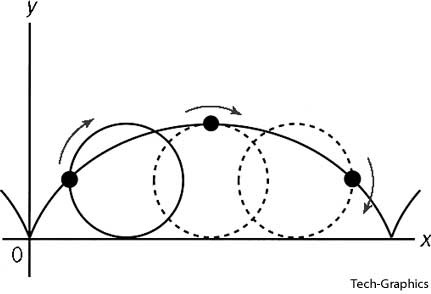
\includegraphics[scale = 0.3]{Cycloid.jpg}
\end{figure}
\end{frame}

\section{Thank You}
\begin{frame}
\centering \Large Thank You!
\end{frame}



\end{document}